%%%
 %
 % Copyright (C) 2019 Ángel Iván Gladín García
 %
 % This program is free software: you can redistribute it and/or modify
 % it under the terms of the GNU General Public License as published by
 % the Free Software Foundation, either version 3 of the License, or
 % (at your option) any later version.
 %
 % This program is distributed in the hope that it will be useful,
 % but WITHOUT ANY WARRANTY; without even the implied warranty of
 % MERCHANTABILITY or FITNESS FOR A PARTICULAR PURPOSE.  See the
 % GNU General Public License for more details.
 %
 % You should have received a copy of the GNU General Public License
 % along with this program.  If not, see <http://www.gnu.org/licenses/>.
%%%

%%%%%%%%%%%%%%%%%%%%%%%%%%%%%%%%%%%%%%%%%%%%%%%%%%%%%%%%%%%%%%%%%%%%%%%%%%%%%%%%%%%%%%%%%
\documentclass[11pt,letterpaper]{article}
\usepackage[utf8]{inputenc}
\usepackage[spanish]{babel}
\usepackage[margin=1in]{geometry}
\usepackage{float}
 
\usepackage{listings}
\usepackage{color}
\usepackage{graphicx}
\usepackage{enumerate}
\usepackage{enumitem}

\usepackage{longtable}
\usepackage{hyperref}
\usepackage{commath}

\usepackage{bbm}
\usepackage{dsfont}
\usepackage{mathrsfs}
\usepackage{amsmath,amsthm,amssymb}
\usepackage{mathtools}
\usepackage{longtable}

%%%%%%%%%%%%%%%%%%%%%%%%%%%%%%%%%%%%%%%%%%%%%%%%%%%%%%%%%%%%%%%%%%%%%%%%%%%%%%%%%%%%%%%%%


%%%%%%%%%%%%%%%%%%%%%%%%%%%%%%%%%%%%%%%%%%%%%%%%%%%%%%%%%%%%%%%%%%%%%%%%%%%%%%%%%%%%%%%%%
\newcommand{\Z}{\mathbb{Z}}
\newcommand{\N}{\mathbb{N}}
\newcommand{\Q}{\mathbb{Q}}
\newcommand{\R}{\mathbb{R}}
\newcommand{\Oh}{\mathcal{O}} %% Notacion "O"
\newcommand{\ent}{\Longrightarrow}
\newcommand{\lra}{\longrightarrow}
\newcommand{\ra}{\rightarrow}
\newcommand{\sii}{\Longleftrightarrow}
\newcommand{\clase}[1]{\overline{#1}}  %% barrita sobre letras
\newcommand{\ord}{\text{ord}}
\newcommand{\leg}[2]{\left( \frac{#1}{#2}\right)} %% Simbolo de Legendre
\newcommand{\sol}{\textbf{\underline{Solución}: }} %% Solución

%%%%%%%%%%%%%%%%%%%%%%%%%%%%%%%%%%%%%%%%%%%%%%%%%%%%%%%%%%%%%%%%%%%%%%%%%%%%%%%%%%%%%%%%%

\begin{document}

%%%%%%%%%%%%%%%%%%%%%%%%%%%%%%%%%%%%%%%%%%%%%%%%%%%%%%%%%%%%%%%%%%%%%%%%%%%%%%%%%%%%%%%%%
\title{
    \vspace{-2cm}
        Universidad Nacional Autónoma de México\\
        Facultad de Ciencias\\
        Criptografía y Seguridad\\
    \vspace{.5cm}
    \large
        \textbf{Reporte de temas a presentar en exposición}\\
        \textbf{Protocolos de seguridad: IPSec, Secure Shell, TLS y PGP}
}
\author{
    Ángel Iván Gladín García\\
    No. cuenta: 313112470\\
    \texttt{angelgladin@ciencias.unam.mx}
}
\date{21 de Mayo 2019}
\maketitle
%%%%%%%%%%%%%%%%%%%%%%%%%%%%%%%%%%%%%%%%%%%%%%%%%%%%%%%%%%%%%%%%%%%%%%%%%%%%%%%%%%%%%%%%%

%%%%%%%%%%%%%%%%%%%%%%%%%%%%%%%%%%%%%%%%%%%%%%%%%%%%%%%%%%%%%%%%%%%%%%%%%%%%%%%%%%%%%%%%%
\newtheorem{theorem}{Teorema}
\newtheorem{example}{Ejemplo}
\newtheorem{corollary}{Corolario}
\newtheorem{lemma}{Lemma}
\newtheorem{definition}{Definición}
\newtheorem{prop}{Proposición}
%%%%%%%%%%%%%%%%%%%%%%%%%%%%%%%%%%%%%%%%%%%%%%%%%%%%%%%%%%%%%%%%%%%%%%%%%%%%%%%%%%%%%%%%%


%%%%%%%%%%%%%%%%%%%%%%%%%%%%%%%%%%%%%%%%%%%%%%%%%%%%%%%%%%%%%%%%%%%%%%%%%%%%%%%%%%%%%%%%%
\section{IPSec (p. 615 - 622)}

Puntos clave:
\begin{itemize}
    \item \textit{IPSec} tiene la capacidad de que puede ser agregado tanto a versión actual del
    protocólo de internet (IPv4 o IPv6) mediante cabeceras adicionales.
    \item \textit{IPSec} abarca tres áreas funcionales: autenticación, confidencialidad y manejo
    de llaves.
    \item La autenticación puede ser aplicada al paquete completo original IP (modo tunel) o a todo
    el paquete a excepción de la cabecera IP.
    \item Se proporciona confidencialidad por un fromato de cifrado conocido como encapsulamiento de
    seguridad del \textit{payload}. Tanto el tunel y los modos de transporte pueden ser adaptados.
\end{itemize}
Implementado seguridad al nivel de IP, una organización puede asegurar interconexión segura, no solo
para las aplicaciones que tienen mecanismos de seguridad también para muchas aplicaciones que no
siguen medidas de seguridad.

Los niveles de seguridad engloban tres áreas operativas:
\begin{itemize}
    \item \textbf{Autenticación}: El mecanismo de autenticación asegura que un paquete recibido era de hecho
    transmitido por uns grupo identificado como la fuente de la cabecera del paquete. Además éste
    mecanismo asegura que que el paquete no ha sido alterado en el camino.
    \item \textbf{Confidencialidad}: La habilidad de la confidencialidad permite que los nodos que se están
    comunicando cifren sus mensajes para prevenir su espionaje por aplicaciones de terceros.
    \item \textbf{Manejo de llaves}: La característica del manejo de llaves se \textit{preocupa} que el
    intercambio de llaves sea seguro.
\end{itemize}

Aplicaciones de IPSec:
IPSec provee la capacidad de tener una comunicación segura a través de LAN, a través de WANs privadas y públicas,
y también a través del internet.
\begin{itemize}
    \item Una conexión segura a internet en surcursales o negocios que dependen mucho en internet y reduce su
    necesidad de hacer una red privada, ahorrándose constos en el manteniento de una red interna.
    \item Un acceso remoto seguro sobre el intenet.
    \item Estableciendo una comunicación \textit{extranet} e \textit{intranet} con una asociación o campañia, esto
    eque IPSec puede ser usado para tener una conexión segura con otra organización, asegurando así la
    autenticación y confidencialidad y proviendo un mecaninso de intercambio de llaves.
    \item Mejorando la seguridad del comercio electrónico, aunque esos portales web ya tengan tengan incluidas
    herramientas de seguridad, IPSec mejora la seguridad. Garantizando que todo el tráfico sea tanto cifrado y
    autenticado, agregando una capa adicional de seguridad.
\end{itemize}

\begin{figure}[H]
    \centering
    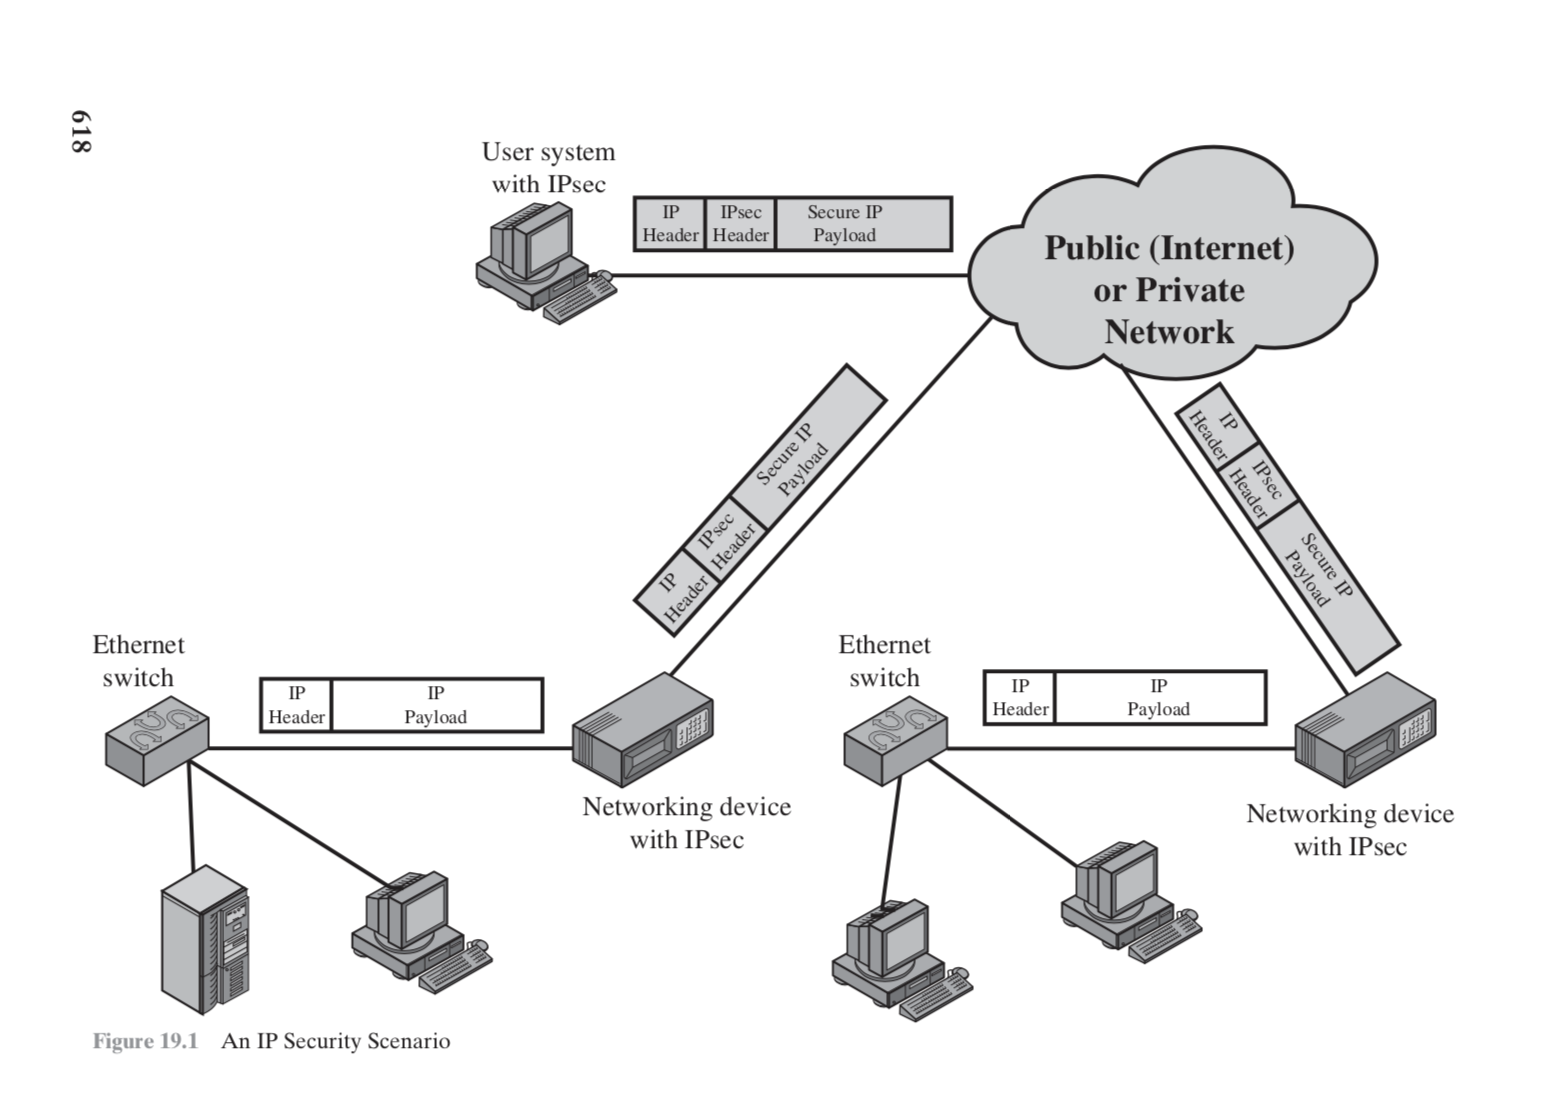
\includegraphics[width=0.7\textwidth]{assets/1.png}
    \caption{Un escenario típico del uso de IPSec.}
\end{figure}

Beneficios de IPSec:
\begin{itemize}
    \item Cuando IPSec es implementado en un \textit{firewall} o en un \textit{router}, provee una fuerte seguridad
    que puede ser aplicado a todo el tráfico.
    \item El \textit{firewall} en IPSec resistente a un \textit{bybass} por tráfico de afuera.
    \item IPSec está por debajo de de la capa de transporte (TCP, UDP) lo que significa que es ``invisible'' para
    las aplicaciones. No hay necesidad de cambiar el \textit{software}.
    \item IPSec puede ser transparente para los usuarios finales. No hay necesidad de entrenar a los usuarios
    en mecanismos de seguridad.
    \item Si se necesita, IPSec puede proveer seguridad individual a los usuarios. Esto es útil para crearles una
    subred privada virtual entre la organización para aplicaciones con contendido sensible. 
\end{itemize}

Documentos IPSec:
La totalidad de la especificaciones IPSec están dispersas entre docenas de RFCs y borradores de documentos IETF. La
mejor forma comprender el alcance de IPSec es consultando la última versión del de IPSec.
El documento puede ser categorizado en los siguientes grupos.
\begin{itemize}
    \item Arquitectura
    \item Cabecera de autenticación (AH)
    \item Encapsulando la seguridad de \textit{payload} (ESP)
    \item Intercambio de llaves de internet (IKE)
    \item Algoritmos criptográficos
    \item Otros
\end{itemize}

Servicios de IPSec:
IPSec provee de servicios de seguridad en la capa de IP permitiendo a un sistema seleccionar los protocolos de
seguridad requeridos, determinar el algoritmo a ser usado para el servicio y poner en su lugar cualquier llave
criptográfica requerida para proveer los servicios solicitados.
\begin{itemize}
    \item Control de accesos
    \item Integridad sin conexión
    \item Autenticación de información de origen
    \item Confidencialidad (cifrado)
    \item Confidencialidad de flujo de tráfico limitado
\end{itemize}


\section{Secure Shell (SSH) (p. 508 - 518)}
\textit{Secure Shell} (SSH) es un protocolo para la comunicación segura de redes diseñado para ser relativamente
simple y que su implementación no sea costosa. La versión incial SSH1 fue enfocada en proveer un mecanismo de
remoto seguro de incio de sesión para remplazar a TELNET y otros clientes remotos de incio de sesión que
proveían seguridad per se.
Una nueva versión, SSH2  arregló muchas fallas de seguridad del esquema original.
Las aplicaciones de cliente y servidor SSH están extensamente disponibles en la gran mayoría de los sistemas
operativos. Ha sido el método de elección para incio de sesión remoto.

SSH está roganizado como tres protocolos que tipicamente se ejecutan encima de TCP.

\begin{figure}[H]
    \centering
    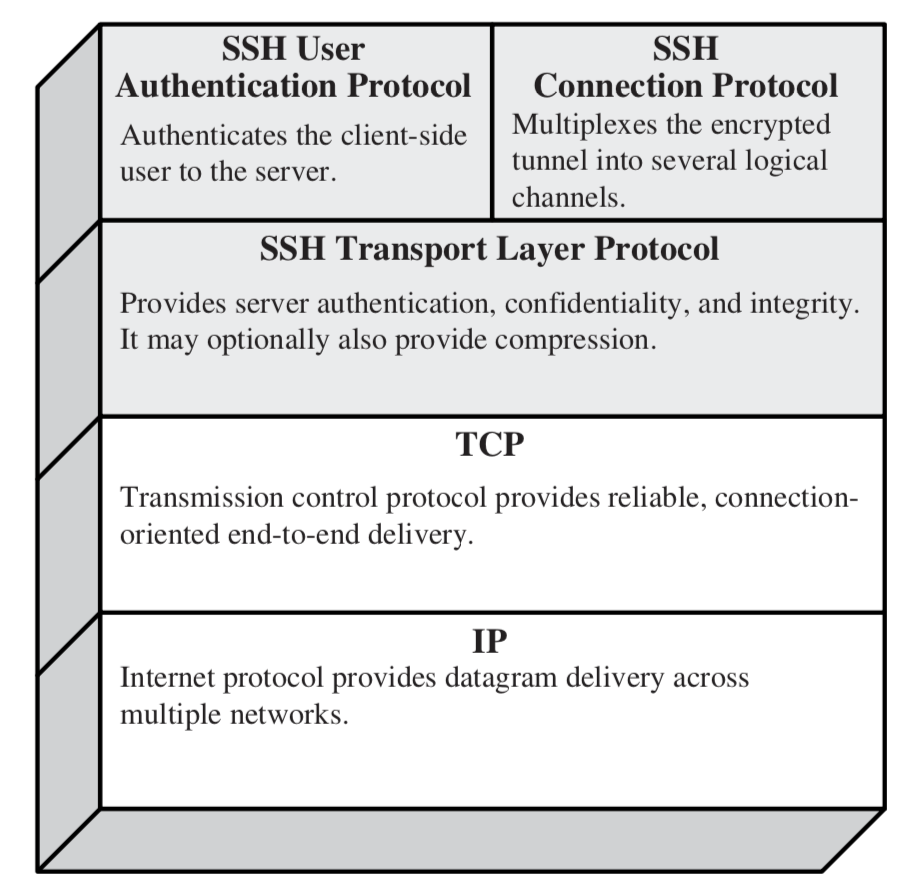
\includegraphics[width=0.4\textwidth]{assets/2.png}
    \caption{Pila de protocolo SSH}
\end{figure}

\begin{itemize}
    \item \textbf{Protocolo de capa de transporte}: Provee autenticación por parte del servidor,
    confidencialidad e integridad de la información conconfidencialidad directa.
    \item \textbf{Protocolo de autenticación de usuario}: Autentica al usuario con el servidor.
    \item \textbf{Protocolo de conexión}: Multiplexa múltiples comunicaciones de canales lógicas sobre
    una sola conección SSH subyacente.
\end{itemize}


\section{Transport Layer Security (TLS) (p. 502 - 506)}
TLS es una inciativa de estandarización de IETF cuya meta es produir una versión de internet
estándar de SSL. TLS es definidos como una propuesta estándar de internet en el RFC 5246. RFC
5246 es muy similar a SSLv3.

Número de versión:
El formato de registro del TLS es el mismo al del SSL 

Código de mensaje de autenticación:
Hay dos diferencias entre los esquemas SSLv3 y el TLS MAC: el algoritmo actual y el alcance del
calculo del MAC. TLS hace uso del algoritmo HMAC definido en RFC2014.

Funciones pseudoaleatorias:
TLS hace uso de funciones pseudoaleatorias concida como PRF para expandir secretos en bloques
de información para fines de generación de llave o validación. El objetico es haaer uso de
un valor secreto relativamente pequeño pero para generar bloques más grandes de información
de forma que sea segura de todo tipo de ataque hecho en una función hasj y MACs.

Código de alerta:
TLS soporta todos los código de alerta definidos en SSLv3 con la excepción de \texttt{no\_certificate}.

Juego de cifrados:
Hay varias pequeñas diferencias entre los juegos de cifrados disponibles sobre SSLv3 y sobre TLS:
\begin{itemize}
    \item \textbf{Intercambio de llave}: TLS soporta todas las técnicas de intercambios de llave de SSLv3
    con la excepción de Fortezza.
    \item \textbf{Algoritmos de cifrado simétrico:} TLS incluye todos los algoritmos de cifrado simétrico 
    encontrados en SSLv3, con la excepción de Fortezza.
\end{itemize}


\section{Pretty Good Privacy (PGP) (p. 568 - 587)}
PGP es un fenómeno notable. En gran parte por el esfuerza de una sola persona, Phil Zimmermann. PGP
provee un servicio de confidencialidad y autenticación que puede ser usado para correo electrónico
y aplicaciones de almacenamiento de archivos. En esenci, Zimmermann hizo lo siguiente:

\begin{itemize}
    \item Seleccionó los mejores algoritmos criptográficos disponibles como bloques de construcción.
    \item Integró esos algoritmos en una aplicación de propósito general que es independiente del 
    sistema operativo y el procesadro, y está basado en un pequeño conjunto de comandos sencillos
    de usar.
    \item Hace el paquete y su documentación, incluyendo el código fuente, libremente disponible en internet.
    \item Entró a un acuerdo con una compañía para proveer compatibilidad completa, un versión
    comercial de bajo costo PGP.
\end{itemize}

PGP ha crecido exponencialmente y ahora es extensamente usada. Un número de sus razones pueden ser citadas
por su crecimiento.

\begin{itemize}
    \item Está disponible libre al rededor del mundo en versiones que pueden ser ejecutadas en nariedad de plataformas
    incluyendo Windows, UNIX, Macintosh y muchas otras más. En adición a ello, la versión comercial satisface 
    a los usuarios que quieren un producto que venga con soporte del vendedor.
    \item Está basado en algoritmos que han sobrevivido a la reseña del público general y son considerados
    extremadamente seguros. Específicamente, el paquete que incluye RSA, DSS, y Diffie-Hellman para cifrado
    de llave pública.
    \item Tiene un amplio rango aplicabilidad para corporaciones que desean seleccionar y mejorar un
    esquema de estandarización para cifrado de archivos y mensajes a individuos que deseen comunicarse 
    seguramente con otros en todo el mundo sobre el internet y otras redes.
    \item No es controlado por ningun gobierno o una organización que da ese estándar.
    \item PGP es ahora un estandar de internet.
\end{itemize}



%%%%%%%%%%%%%%%%%%%%%%%%%%%%%%%%%%%%%%%%%%%%%%%%%%%%%%%%%%%%%%%%%%%%%%%%%%%%%%%%%%%%%%%%%


%%%%%%%%%%%%%%%%%%%%%%%%%%%%%%%%%%%%%%%%%%%%%%%%%%%%%%%%%%%%%%%%%%%%%%%%%%%%%%%%%%%%%%%%%
\begin{thebibliography}{}

\bibitem{}
Stallings, William,
\textit{Cryptography and Network Security: Principles and Practice},
5a Ed., Pretince Hall, 2010.

\end{thebibliography}
%%%%%%%%%%%%%%%%%%%%%%%%%%%%%%%%%%%%%%%%%%%%%%%%%%%%%%%%%%%%%%%%%%%%%%%%%%%%%%%%%%%%%%%%%

\end{document}
